% paper_arxiv.tex — arXiv preprint version
\documentclass[11pt,a4paper]{article}

% ── Geometry ──────────────────────────────────────────────────────────────
\usepackage[margin=1.15in,top=1in,bottom=1in]{geometry}

% ── Mathematics ───────────────────────────────────────────────────────────
\usepackage{amsmath,amssymb,amsthm,mathtools}

% ── Fonts (Computer Modern — standard arXiv) ─────────────────────────────
\usepackage[T1]{fontenc}
\usepackage{lmodern}
\usepackage{microtype}

% ── Tables and figures ────────────────────────────────────────────────────
\usepackage{booktabs}
\usepackage{graphicx}
\graphicspath{{../figures/}}
\usepackage{caption}
\usepackage{subcaption}
\usepackage{float}

% ── References and links ─────────────────────────────────────────────────
\usepackage[dvipsnames]{xcolor}
\usepackage[colorlinks,linkcolor=MidnightBlue,citecolor=MidnightBlue,
            urlcolor=MidnightBlue]{hyperref}
\usepackage[capitalise,noabbrev]{cleveref}

% ── Misc ──────────────────────────────────────────────────────────────────
\usepackage{enumitem}
\usepackage{textcomp}

% ── Theorem environments ─────────────────────────────────────────────────
\theoremstyle{plain}
\newtheorem{theorem}{Theorem}
\newtheorem{proposition}[theorem]{Proposition}
\newtheorem{lemma}[theorem]{Lemma}
\newtheorem{corollary}[theorem]{Corollary}

\theoremstyle{definition}
\newtheorem{definition}[theorem]{Definition}
\newtheorem{assumption}[theorem]{Assumption}
\newtheorem{example}[theorem]{Example}

\theoremstyle{remark}
\newtheorem{remark}[theorem]{Remark}

% ── Notation shortcuts ───────────────────────────────────────────────────
\DeclareMathOperator*{\argmax}{arg\,max}
\newcommand{\R}{\mathbb{R}}
\newcommand{\abs}[1]{\lvert #1 \rvert}
\newcommand{\norm}[1]{\lVert #1 \rVert}

% ══════════════════════════════════════════════════════════════════════════
\begin{document}

\title{Product Modification, Legal Pricing Constraints,\\ and Third-Degree Price Discrimination}

\author{%
  Sophia Ng\thanks{Department of Economics, University of Toronto. \texttt{sophia.ng@mail.utoronto.ca}}
  \and
  Sohail (Neel) Sarkar\thanks{Department of Mathematics, University of Toronto. \texttt{sohail.sarkar@mail.utoronto.ca}}
}

\date{March 2026}

\maketitle

% ── Abstract ─────────────────────────────────────────────────────────────
\begin{abstract}
We study how a monopolist manufacturer circumvents a common-wholesale-price constraint by introducing low-cost product variants.
In a two-retailer linear-demand model, a legal constraint (modeled on the Robinson--Patman Act) forces a single wholesale price for identical goods.
The manufacturer can pay a per-unit cost $k\ge 0$ to create differentiated variants, restoring segment-specific pricing.
We derive closed-form profit under both regimes, prove that variant-based discrimination is strictly profitable for generic parameter values when $k=0$, characterize the threshold cost $\bar{k}$ as a function of demand heterogeneity and expected legal penalty $L$, and verify the standard Ramsey inverse-elasticity condition at the discriminatory optimum.
Welfare analysis shows the output condition of Schmalensee (1981) extends to this setting, with an additional social cost $k\sum_i Q_i^D$ when $k>0$.
We provide descriptive evidence using 3.24\,M scanner observations from Dominick's Finer Foods: OLS of per-unit price on $\ln(\text{Size})$ yields $\hat\beta = -3.00$ ($\text{SE}=0.37$); store fixed effects are jointly significant ($F=15.04$); within-brand regressions for Tide, All, and Purex confirm the gradient persists within product lines.
\end{abstract}

\smallskip
\noindent\textit{Keywords:} price discrimination, nonlinear pricing, legal constraints, product differentiation, scanner data

\smallskip
\noindent\textit{MSC 2020:} 91B24, 91B26 \quad\textit{JEL:} D42, L11, L42, K21

\bigskip


% ══════════════════════════════════════════════════════════════════════════
\section{Introduction}\label{sec:intro}

Third-degree price discrimination requires that a firm charge different prices to distinct market segments.
The classical treatment~\cite{Pigou1920,Varian1989} assumes the firm can freely partition markets and set segment-specific prices.
In many jurisdictions, however, wholesale price discrimination is legally constrained.
In the United States, the Robinson--Patman Act (RPA, 1936) prohibits charging competing buyers different prices for commodities of ``like grade and quality''~\cite{FTC_RPA}.

Manufacturers respond by introducing \emph{product variants}---differences in package size, labeling, or minor formulation---that place goods outside the ``like grade and quality'' category, effectively relaxing the uniform-price constraint.
The Seventh Circuit's decision in \emph{Woodman's Food Market v.\ Clorox}~\cite{Woodmans2016} illustrates the legal significance of this boundary.
Despite its practical importance, the product-modification channel has received limited formal treatment.
Yonezawa, G\'omez, and Richards~\cite{Yonezawa2020} document wholesale-price divergence across retailers but do not model the mechanism.
Kobayashi and Muris~\cite{KobayashiMuris2026} analyze the economics of Robinson--Patman from a policy perspective.
Ross~\cite{CBSWinners} studies the Act's distributional effects.

\paragraph{Contributions.}
We make three contributions.
\begin{enumerate}[nosep,label=(\roman*)]
\item A tractable model in which product modification is an explicit decision variable interacting with a common-price legal constraint (\cref{sec:model}).
\item Closed-form expressions for the profit gain, threshold differentiation cost $\bar{k}$, and comparative statics in the legal penalty $L$ (\cref{prop:profit,prop:threshold}).
\item Descriptive evidence from 3.24\,M scanner observations linking the model's predictions to observed size--price gradients and within-brand pricing patterns (\cref{sec:empirical}).
\end{enumerate}


% ══════════════════════════════════════════════════════════════════════════
\section{Model}\label{sec:model}

\subsection{Environment}

A monopolist manufacturer with constant marginal cost $c>0$ supplies two retailers $i\in\{1,2\}$.
Retailer $i$ faces linear demand
\begin{equation}\label{eq:demand}
  Q_i(p_i) = a_i - b_i\,p_i, \qquad a_i,\,b_i > 0,
\end{equation}
and applies a fixed markup $m_i\ge 0$, so $p_i = w_i + m_i$.
Without loss of generality, $b_1 < b_2$ (retailer~1 has less elastic demand).

\begin{assumption}[Legal constraint]\label{ass:rpa}
When the manufacturer sells identical commodities to both retailers, it must charge a common wholesale price $w_1=w_2=w$.
If it introduces distinct variants at per-unit cost $k\ge 0$, it may set $w_1\ne w_2$.
\end{assumption}

The timing is: (i)~the manufacturer chooses a pricing/product-design strategy; (ii)~retailers observe wholesale prices and set retail prices $p_i = w_i + m_i$.

\subsection{Uniform-pricing regime}\label{sec:uniform}

Under the legal constraint, the manufacturer solves
\begin{equation}\label{eq:pi_u_fn}
  \max_{w}\; \Pi^U(w) = (w-c)\sum_{i=1}^{2}\bigl(a_i - b_i(w+m_i)\bigr).
\end{equation}
This is a concave quadratic in $w$, with unique maximizer
\begin{equation}\label{eq:wstar}
  w^* = \frac{\sum_i(a_i - b_i m_i) + c\sum_i b_i}{2\sum_i b_i}
\end{equation}
and optimal profit
\begin{equation}\label{eq:pi_u}
  \Pi^U = \frac{\bigl(\sum_i(a_i - b_i m_i) - c\sum_i b_i\bigr)^2}{4\sum_i b_i}.
\end{equation}

\subsection{Discriminatory regime}\label{sec:discrim}

With distinct variants, the manufacturer independently maximizes over each $w_i$:
\begin{equation}\label{eq:pi_d_fn}
  \Pi^D(w_1,w_2;\,k) = \sum_{i=1}^{2}(w_i - c - k)\bigl(a_i - b_i(w_i + m_i)\bigr).
\end{equation}
The first-order conditions yield
\begin{equation}\label{eq:wi}
  w_i^* = \frac{a_i - b_i m_i + b_i(c+k)}{2b_i} = \frac{a_i}{2b_i} - \frac{m_i}{2} + \frac{c+k}{2},
\end{equation}
with optimal profit
\begin{equation}\label{eq:pi_d}
  \Pi^D(k) = \sum_{i=1}^{2}\frac{\bigl(a_i - b_i m_i - b_i(c+k)\bigr)^2}{4b_i}.
\end{equation}
We maintain $k < \min_i\hat{k}_i$, where $\hat{k}_i \coloneqq a_i/b_i - m_i - c$, so that both markets are served.

\subsection{Main results}

\begin{proposition}[Strict profitability]\label{prop:profit}
Under linear demand with fixed markups, if\/
$\frac{a_1 - b_1 m_1}{b_1} \ne \frac{a_2 - b_2 m_2}{b_2}$
and $k=L=0$, then $\Pi^D(0) > \Pi^U$.
\end{proposition}

\begin{proof}
Under discrimination with $k=0$, the manufacturer solves two independent concave programs, obtaining $w_i^*$ from~\eqref{eq:wi}.
These coincide at a single $w$ if and only if
\[
  \frac{a_1 - b_1 m_1}{b_1} = \frac{a_2 - b_2 m_2}{b_2},
\]
which holds on a Lebesgue-measure-zero set of $(a_i,b_i,m_i)$.
Under the stated inequality, $w_1^*\ne w_2^*$, and the constraint $w_1=w_2$ is binding.
By the envelope theorem, the constrained maximum of a smooth objective is strictly less than the unconstrained maximum when the constraint binds.
\end{proof}

\begin{remark}\label{rem:generic}
The condition in \cref{prop:profit} is generic: when $b_1\ne b_2$, equality of the two ratios requires a knife-edge restriction on the remaining parameters.
\end{remark}

Since $\Pi^D(k)$ is strictly decreasing and continuous in $k$ with $\Pi^D(0)>\Pi^U$, there exists a unique threshold $\bar{k}>0$ satisfying
\begin{equation}\label{eq:threshold}
  \Pi^D(k) > \Pi^U \;\Longleftrightarrow\; k < \bar{k}.
\end{equation}

\begin{proposition}[Threshold and comparative statics]\label{prop:threshold}
There exists $\bar{k}>0$ such that, for sufficiently small expected legal penalty $L\ge 0$, the manufacturer prefers variant-based discrimination iff $k<\bar{k}$.
Moreover:
\begin{enumerate}[nosep,label=(\alph*)]
  \item $\bar{k}$ is increasing in $\abs{b_1-b_2}$;
  \item $\bar{k}$ is decreasing in $L$.
\end{enumerate}
\end{proposition}

\begin{proof}
Differentiating~\eqref{eq:pi_d}:
$\partial\Pi^D/\partial k = -\tfrac{1}{2}\sum_i(a_i - b_i m_i - b_i(c+k)) < 0$
for $k<\min_i\hat{k}_i$.
Continuity, strict monotonicity, and $\Pi^D(0)>\Pi^U$ yield a unique $\bar{k}\in(0,\min_i\hat{k}_i)$ with $\Pi^D(\bar{k})=\Pi^U$.

(a)~$\Pi^D(0)-\Pi^U$ increases in $\abs{b_1-b_2}$, since greater heterogeneity makes the uniform-price compromise costlier, raising $\bar{k}$.

(b)~With legal risk, the break-even condition becomes $\Pi^D(\bar{k})=\Pi^U+L$. Since $\Pi^D$ is decreasing, increasing $L$ tightens the threshold.
\end{proof}

\paragraph{Closed form for $\bar{k}$.}
Define $S_i(k)\coloneqq a_i - b_i m_i - b_i(c+k)$, $\Sigma\coloneqq\sum_i b_i$, and $R\coloneqq\sum_i(a_i-b_im_i)-c\Sigma$.
Then $\bar{k}$ solves the quadratic
\begin{equation}\label{eq:kbar_quadratic}
  \frac{\Sigma}{4}\,\bar{k}^2
  - \frac{1}{2}\Bigl(\sum_i S_i(0)\Bigr)\bar{k}
  + \Bigl[\sum_i\frac{S_i(0)^2}{4b_i} - \frac{R^2}{4\Sigma} - L\Bigr] = 0.
\end{equation}
The economically relevant root is the smaller positive solution.

\subsection{Ramsey pricing at the optimum}\label{sec:ramsey}

At the discriminatory equilibrium, the price elasticity in segment $i$ is $\varepsilon_i = -b_i\,p_i^D/Q_i^D$, and the optimal pricing rule satisfies
\begin{equation}\label{eq:ramsey}
  \frac{p_i^D - (c+k)}{p_i^D} = \frac{1}{\abs{\varepsilon_i}},
\end{equation}
the standard Ramsey inverse-elasticity condition~\cite{Varian1989}.


% ══════════════════════════════════════════════════════════════════════════
\section{Welfare}\label{sec:welfare}

Under linear demand, consumer surplus in segment $i$ at price $p_i$ is $CS_i = Q_i^2/(2b_i)$.
Total welfare under each regime:
\begin{align}
  W^U &= \sum_{i}\Bigl[\frac{(Q_i^U)^2}{2b_i} + (p_i^U - c)\,Q_i^U\Bigr], \label{eq:wu}\\
  W^D &= \sum_{i}\Bigl[\frac{(Q_i^D)^2}{2b_i} + (p_i^D - c - k)\,Q_i^D\Bigr]. \label{eq:wd}
\end{align}
The standard output condition~\cite{Schmalensee1981} extends to this setting:
\begin{equation}\label{eq:welfare_condition}
  W^D \ge W^U \;\Longleftrightarrow\; \sum_i Q_i^D \ge \sum_i Q_i^U.
\end{equation}
Substituting:
\begin{equation}\label{eq:output_condition}
  \sum_i Q_i^D - \sum_i Q_i^U = \sum_i b_i(w^* - w_i^*).
\end{equation}
The sign depends on parameter values; discrimination does not unambiguously raise or lower welfare.

\begin{remark}[Welfare cost of differentiation]\label{rem:k_welfare}
When $k>0$, the real resource cost $k\sum_i Q_i^D$ must be subtracted from $W^D$.
The output condition~\eqref{eq:welfare_condition} then becomes necessary but not sufficient; the output expansion must dominate the differentiation cost.
\end{remark}


% ══════════════════════════════════════════════════════════════════════════
\section{Empirical Evidence}\label{sec:empirical}

\subsection{Data}

We use the Dominick's Finer Foods scanner dataset~\cite{Dominicks}, a panel of store-week-UPC retail transactions from a Chicago-area supermarket chain.
The laundry-detergent category yields $n=3{,}240{,}409$ observations spanning 566 UPCs, 93 stores, and 396 weeks after standard cleaning.\footnote{%
  Observations with zero price, zero movement, or quality-flag failures are dropped.
  Per-unit prices in the top/bottom 0.1\% are trimmed.
  Package sizes are converted to fluid ounces; non-convertible units (loads, count) excluded.}
Brands are extracted via string matching; a binary sale indicator flags promotional weeks.

\subsection{Specification}

The dependent variable is per-unit price in cents per ounce:
\begin{equation}\label{eq:ppu}
  \mathrm{ppu}_{ijt} = \frac{\mathrm{Price}_{ijt}/\mathrm{QTY}_{ijt}}{\mathrm{Size}_i}\times 100.
\end{equation}
We estimate
\begin{equation}\label{eq:reg}
  \mathrm{ppu}_{ijt}
    = \alpha + \beta\,\ln(\mathrm{Size}_i)
    + \gamma_j + \delta_b + \phi\,\mathbf{1}[\mathrm{Sale}_{ijt}]
    + \varepsilon_{ijt},
\end{equation}
where $\gamma_j$ and $\delta_b$ are store and brand fixed effects.
Standard errors are clustered by UPC (566 clusters).

\subsection{Results}

\Cref{tab:regression} reports four specifications.

\begin{table}[htbp]
\centering
\caption{Per-Unit Price Regressions: Dominick's Laundry Detergent}
\label{tab:regression}
\small
\begin{tabular}{lcccc}
\toprule
 & (1) & (2) & (3) & (4) \\
\midrule
$\ln(\text{Size})$ & $-3.003^{***}$ & $-3.007^{***}$ & $-2.820^{***}$ & $-2.800^{***}$ \\
 & $(0.369)$ & $(0.369)$ & $(0.366)$ & $(0.367)$ \\
[4pt]
Sale indicator &  &  &  & $-0.606^{***}$ \\
 &  &  &  & $(0.079)$ \\
[4pt]
Constant & $20.069^{***}$ & $20.405^{***}$ & $17.582^{***}$ & $17.613^{***}$ \\
 & $(1.656)$ & $(1.663)$ & $(1.623)$ & $(1.624)$ \\
\midrule
Store FE & No & Yes & Yes & Yes \\
Brand FE & No & No & Yes & Yes \\
\midrule
$R^2$ & 0.382 & 0.385 & 0.470 & 0.474 \\
Adj.\ $R^2$ & 0.382 & 0.385 & 0.470 & 0.474 \\
$N$ & 3,240,409 & 3,240,409 & 3,240,409 & 3,240,409 \\
\bottomrule
\end{tabular}

\medskip\par\noindent\footnotesize
\textit{Notes:} Dependent variable is per-unit price in cents per ounce. Standard errors clustered by UPC in parentheses. $^{***}\,p<0.01$, $^{**}\,p<0.05$, $^{*}\,p<0.10$. Store FE: 93 store dummies. Brand FE: 23 brand dummies.
\end{table}


\noindent
Key findings:
\begin{enumerate}[nosep,label=(\roman*)]
\item \textbf{Size gradient.}
  Baseline: $\hat\beta=-3.003$ (SE\,$=0.369$, $p<0.001$), $R^2=0.382$.
  A one-log-unit increase in size (roughly $\times 2.7$) is associated with a 3.0\,\textcent/oz decrease in per-unit price.
\item \textbf{Store heterogeneity.}
  Joint $F$-test on 92 store dummies: $F=15.04$ ($p<0.001$).
  Cross-store variation persists after controlling for size and brand.
  Dominick's operated 16 pricing zones collapsing into four tiers~\cite{DominicksManual}; store FE capture a mixture of zone policy and local demand.
\item \textbf{Brand effects.}
  Adding brand FE raises $R^2$ from 0.385 to 0.470 ($\Delta R^2\approx 0.09$); $\hat\beta$ attenuates to $-2.820$.
  The residual within-brand size gradient remains large and significant.
\item \textbf{Sale control.}
  The sale indicator enters at $-0.606$ (SE\,$=0.079$).
  $\hat\beta$ is robust at $-2.800$.
\end{enumerate}

\paragraph{Robustness.}
\Cref{tab:robustness} re-estimates the full specification under store-level and two-way (UPC$\times$store) clustering~\cite{CGM2011}.
Point estimates are unchanged.
Under two-way clustering, standard errors are close to the UPC-only baseline, indicating that UPC-level dependence dominates.

% generated by robustness_table.py
\begin{table}[H]
\centering
\caption{Robustness Checks: Alternative Clustering Schemes (Full Model)}
\label{tab:robustness}
\begin{tabular}{lccc}
\toprule
 & (1) & (2) & (3) \\
 & UPC Clustered & Store Clustered & Two-Way Clustered \\
 & & & (UPC $\times$ Store) \\
\midrule
$\ln(\text{Size})$ & -2.800*** & -2.800*** & -2.800*** \\
 & (0.367) & (0.012) & (0.365) \\[4pt]
Sale indicator & -0.606*** & -0.606*** & -0.606*** \\
 & (0.079) & (0.015) & (0.080) \\[4pt]
\midrule
Store FE    & \checkmark & \checkmark & \checkmark \\
Brand FE    & \checkmark & \checkmark & \checkmark \\
$R^{2}$     & 0.474 & 0.474 & 0.474 \\
$N$         & \multicolumn{3}{c}{3,240,409} \\
\bottomrule
\multicolumn{4}{p{0.88\textwidth}}{\footnotesize \textit{Notes:}
Dependent variable: per-unit price (cents/oz). All three columns use
the same OLS regression with store and brand fixed effects; only the
covariance estimator differs. Cluster-robust standard errors in
parentheses. Column~(3) applies the Cameron, Gelbach, and Miller
(2011) two-way formula:
$\hat{V}_{\text{two-way}} =
 \hat{V}_{\text{UPC}} + \hat{V}_{\text{Store}}
 - \hat{V}_{\text{UPC}\times\text{Store}}$.
Point estimates are identical across columns.
$^{***}p<0.01$, $^{**}p<0.05$, $^{*}p<0.10$.}
\end{tabular}
\end{table}


\paragraph{Within-brand regressions.}
\Cref{tab:within_brand} restricts the sample to Tide, All, and Purex separately.
The size gradient persists within each brand ($\hat\beta_{\text{Tide}}=-0.74$, $\hat\beta_{\text{All}}=-1.22$, $\hat\beta_{\text{Purex}}=-3.13$; all $p<0.01$), ruling out across-brand composition as the sole driver.

\begin{table}[htbp]
\centering
\caption{Within-Brand Size--Price Gradient}
\label{tab:within_brand}
\small
\begin{tabular}{lccc}
\toprule
 & Tide & All & Purex \\
\midrule
$\ln(\text{Size})$ & $-0.740^{***}$ & $-1.223^{***}$ & $-3.129^{***}$ \\
 & $(0.178)$ & $(0.401)$ & $(0.817)$ \\
[4pt]
Sale indicator & $-0.808^{***}$ & $-0.186$ & $-0.425^{*}$ \\
 & $(0.077)$ & $(0.130)$ & $(0.255)$ \\
\midrule
Store FE & Yes & Yes & Yes \\
\midrule
$R^2$ & 0.231 & 0.209 & 0.492 \\
Adj.\ $R^2$ & 0.230 & 0.209 & 0.492 \\
$N$ & 564,067 & 237,357 & 104,329 \\
UPCs & 78 & 51 & 22 \\
\bottomrule
\end{tabular}

\medskip\par\noindent\footnotesize
\textit{Notes:} Dependent variable is per-unit price in cents per ounce. Each column restricts the sample to a single brand. Standard errors clustered by UPC in parentheses. $^{***}\,p<0.01$, $^{**}\,p<0.05$, $^{*}\,p<0.10$. All specifications include store fixed effects and a sale indicator.
\end{table}


\paragraph{Placebo.}
\Cref{tab:placebo} regresses both per-unit price and total shelf price on $\ln(\text{Size})$.
The coefficient is strongly negative for per-unit price ($-2.80$) and strongly positive for shelf price ($+3.89$), confirming a quantity-discount schedule rather than a mechanical artefact.

\begin{table}[htbp]
\centering
\caption{Placebo Check: Per-Unit Price vs.\ Total Shelf Price}
\label{tab:placebo}
\small
\begin{tabular}{lcc}
\toprule
 & (1) PPU (\textcent/oz) & (2) Shelf price (\$) \\
\midrule
$\ln(\text{Size})$ & $-2.800^{***}$ & $3.893^{***}$ \\
 & $(0.367)$ & $(0.303)$ \\
[4pt]
Sale indicator & $-0.606^{***}$ & $-0.662^{***}$ \\
 & $(0.079)$ & $(0.088)$ \\
\midrule
Store FE & Yes & Yes \\
Brand FE & Yes & Yes \\
\midrule
$R^2$ & 0.474 & 0.652 \\
Adj.\ $R^2$ & 0.474 & 0.652 \\
$N$ & 3,240,409 & 3,240,409 \\
\bottomrule
\end{tabular}

\medskip\par\noindent\footnotesize
\textit{Notes:} Column~(1) uses per-unit price (cents per ounce) as the dependent variable. Column~(2) uses total shelf price (dollars). The negative coefficient in column~(1) and the positive coefficient in column~(2) confirm that larger packages have lower per-unit prices but higher total prices, ruling out a mechanical coding artefact. Standard errors clustered by UPC in parentheses. $^{***}\,p<0.01$, $^{**}\,p<0.05$, $^{*}\,p<0.10$.
\end{table}


\subsection{Limitations}

The Dominick's data cover a single retail chain; we observe within-chain variation rather than the cross-chain discrimination central to Robinson--Patman.
Wholesale prices are unobserved.
Package size is endogenous.
Ounce-based normalisation may not equalize washing capacity across formulations; load-equivalent pricing would be more rigorous but load counts are unavailable.
The Dominick's data do not observe wholesale contracts, retailer-specific manufacturer variants, or cross-chain product allocation.
Accordingly, the evidence documents retail pricing patterns \emph{consistent with} the model's mechanism but does not directly test the wholesale discrimination channel.
Causal identification would require an instrument for package-size choices or matched wholesale--retail data spanning multiple chains.


% ══════════════════════════════════════════════════════════════════════════
\section{Discussion}\label{sec:discussion}

The model and data are motivated by the institutional setting of the Robinson--Patman Act, but the formal structure is more general: any common-price constraint that a firm can relax via low-cost product differentiation produces the same trade-off between differentiation cost $k$, profit gain, and legal risk $L$.

Relevant applications include:
\begin{itemize}[nosep]
  \item \emph{Detergent packaging.} Manufacturers offer sizes from 50\,oz to 400\,oz; the Dominick's data show per-unit prices ranging from 5 to 12\,\textcent/oz within Tide alone.
  \item \emph{Branded vs.\ authorized generics.} Chemically identical pharmaceuticals sold under distinct trade dress correspond to variants $A$, $B$ with different demand parameters.
  \item \emph{Retailer-exclusive SKUs.} Mattress models with cosmetic differences (quilting, fabric covers) create retailer-specific UPCs, raising search costs and sustaining price dispersion.
  \item \emph{International editions.} Textbook publishers sell downgraded editions in elastic foreign markets, using physical differences to segment and limit arbitrage.
\end{itemize}

From a welfare perspective, variant-based discrimination can expand output in elastic segments but sustains higher prices in inelastic ones.
The net effect depends on whether total output rises~\cite{Schmalensee1981,Varian1989}.
When $k>0$, the social cost of differentiation further erodes the potential welfare gain (\cref{rem:k_welfare}).
Enforcement narrowly targeting ``identical commodities'' may therefore induce \emph{more} cosmetic differentiation rather than less discrimination.


% ══════════════════════════════════════════════════════════════════════════
\section{Conclusion}\label{sec:conclusion}

We model how product modification enables a manufacturer to circumvent a common-wholesale-price constraint and implement third-degree price discrimination.
Closed-form results characterize the profit gain, threshold cost $\bar{k}$, and Ramsey pricing at the optimum.
Scanner data covering 3.24\,M laundry-detergent transactions yield a steep size--price gradient ($\hat\beta=-3.0$), significant store heterogeneity ($F=15.04$), and persistent within-brand gradients.
Extensions to endogenous retailer pricing, multi-chain data, and instrumental-variable identification are left for future work.


% ══════════════════════════════════════════════════════════════════════════
\appendix

\section{Asymmetric markups}\label{app:robustness}

With $m_1\ne m_2$, the uniform-price optimum becomes
$w^*=\frac{(a_1+a_2)-(b_1 m_1+b_2 m_2)+c(b_1+b_2)}{2(b_1+b_2)}$
and the discriminatory optima remain $w_i^*=\frac{a_i-b_im_i+b_i(c+k)}{2b_i}$.
The profit gain $\Pi^D(0)-\Pi^U>0$ whenever $w_1^*\ne w_2^*$, which is generically satisfied when $b_1\ne b_2$ or $m_1\ne m_2$.
All comparative statics carry through.

\section{Simulation figures}\label{app:sim}

\begin{figure}[H]
\centering
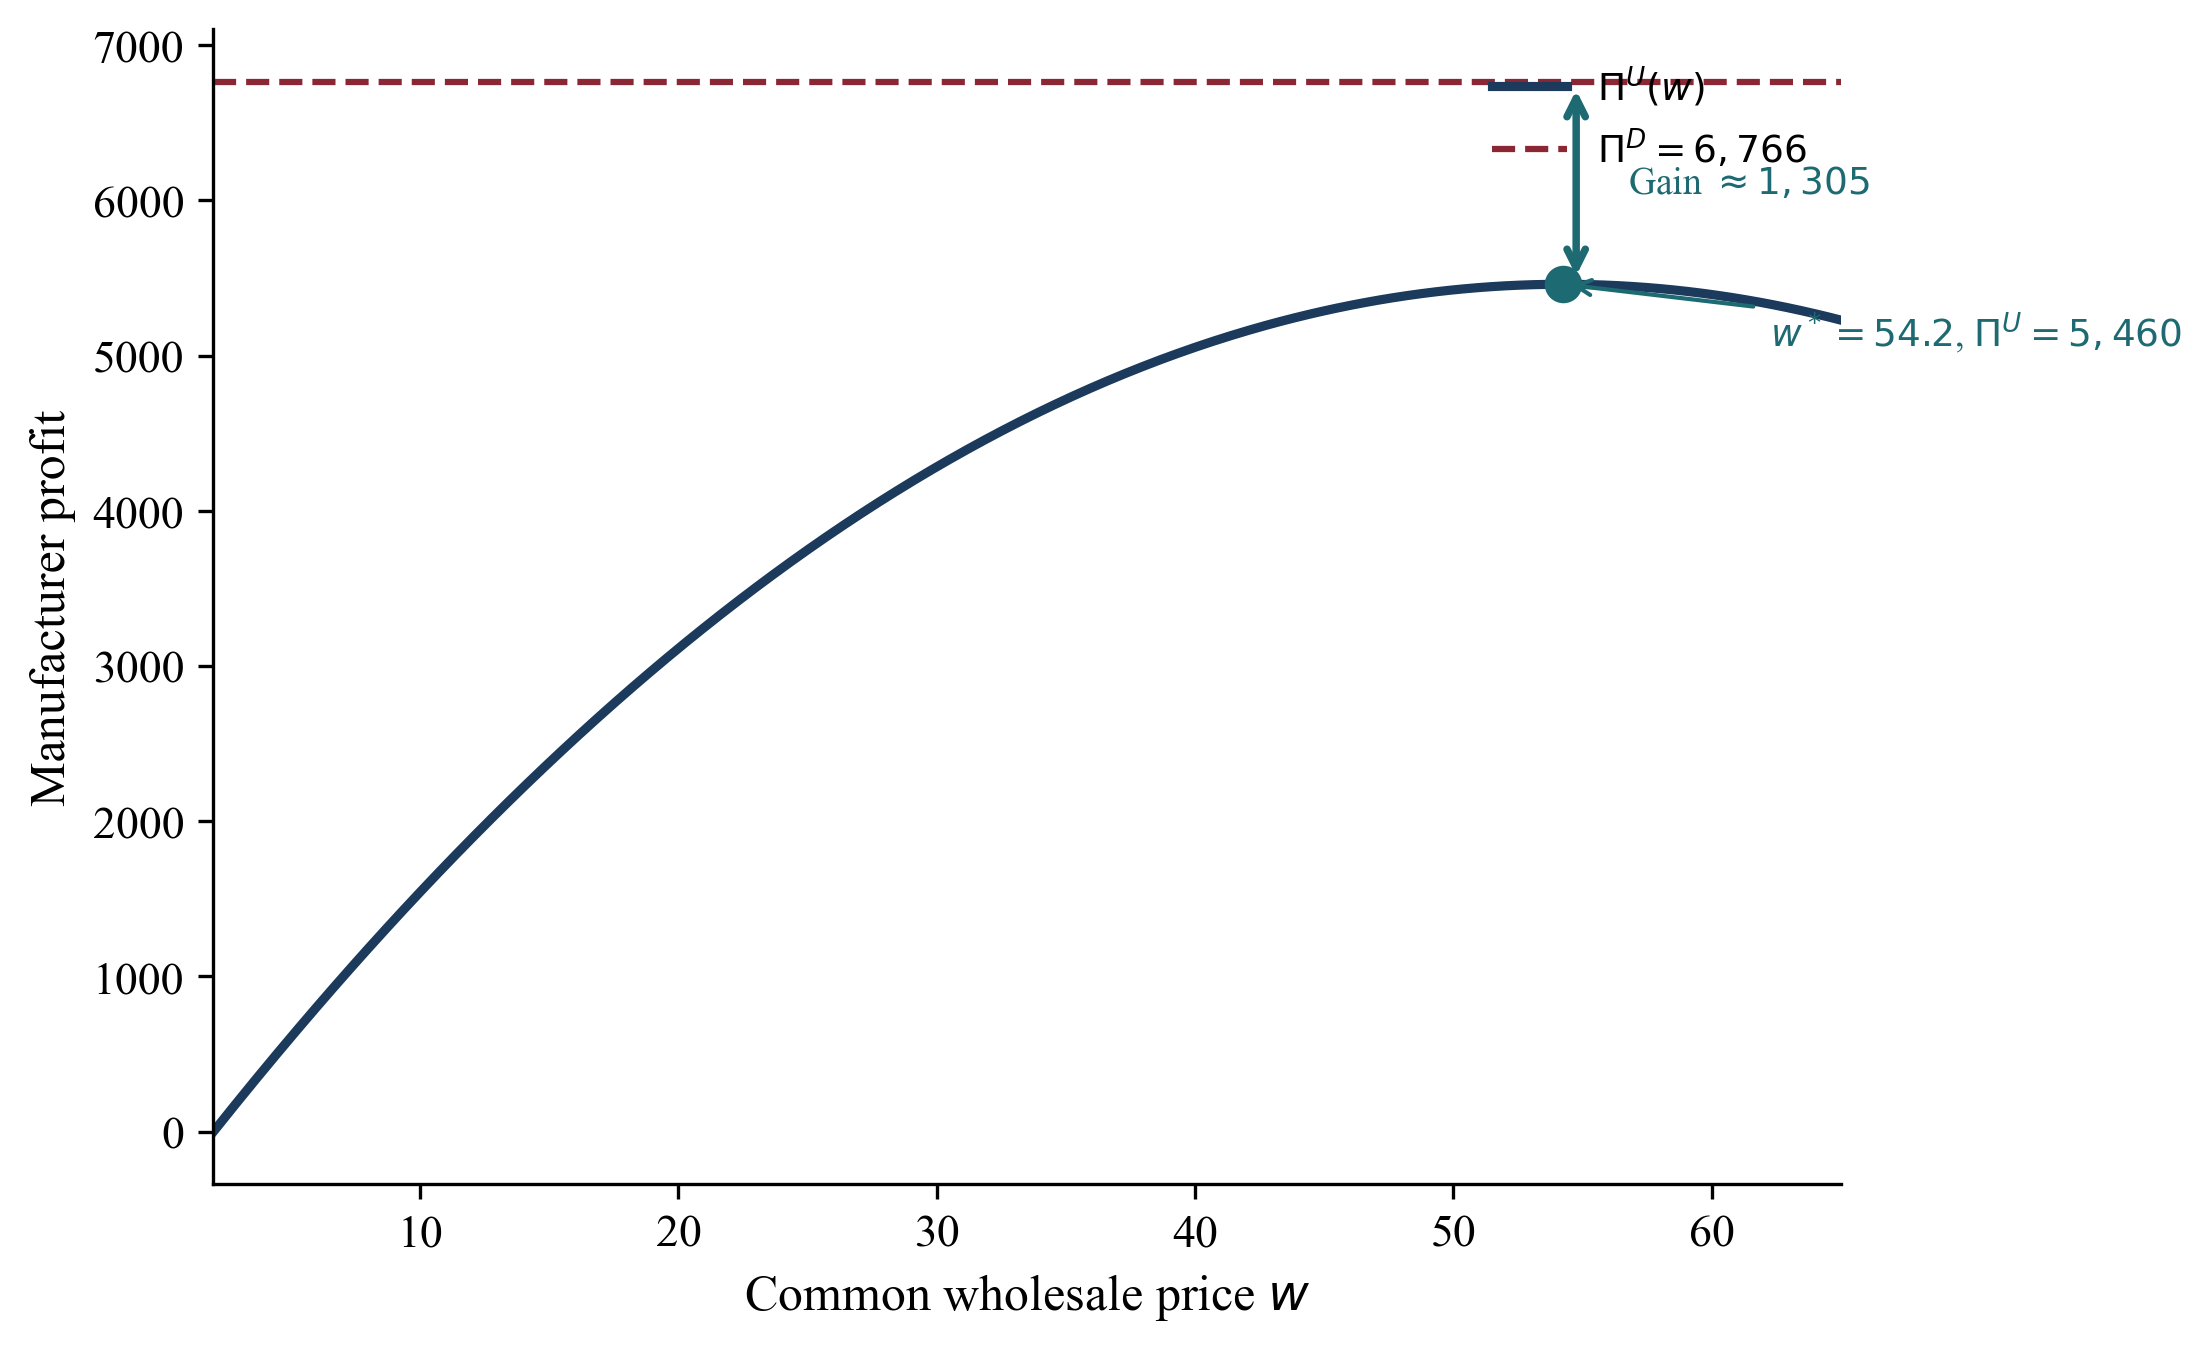
\includegraphics[width=0.75\textwidth]{fig1_profit_curve.png}
\caption{Manufacturer profit $\Pi^U(w)$ under uniform pricing.
Dashed line: $\Pi^D$ under variant-based discrimination.}
\label{fig:profit_curve}
\end{figure}

\begin{figure}[H]
\centering
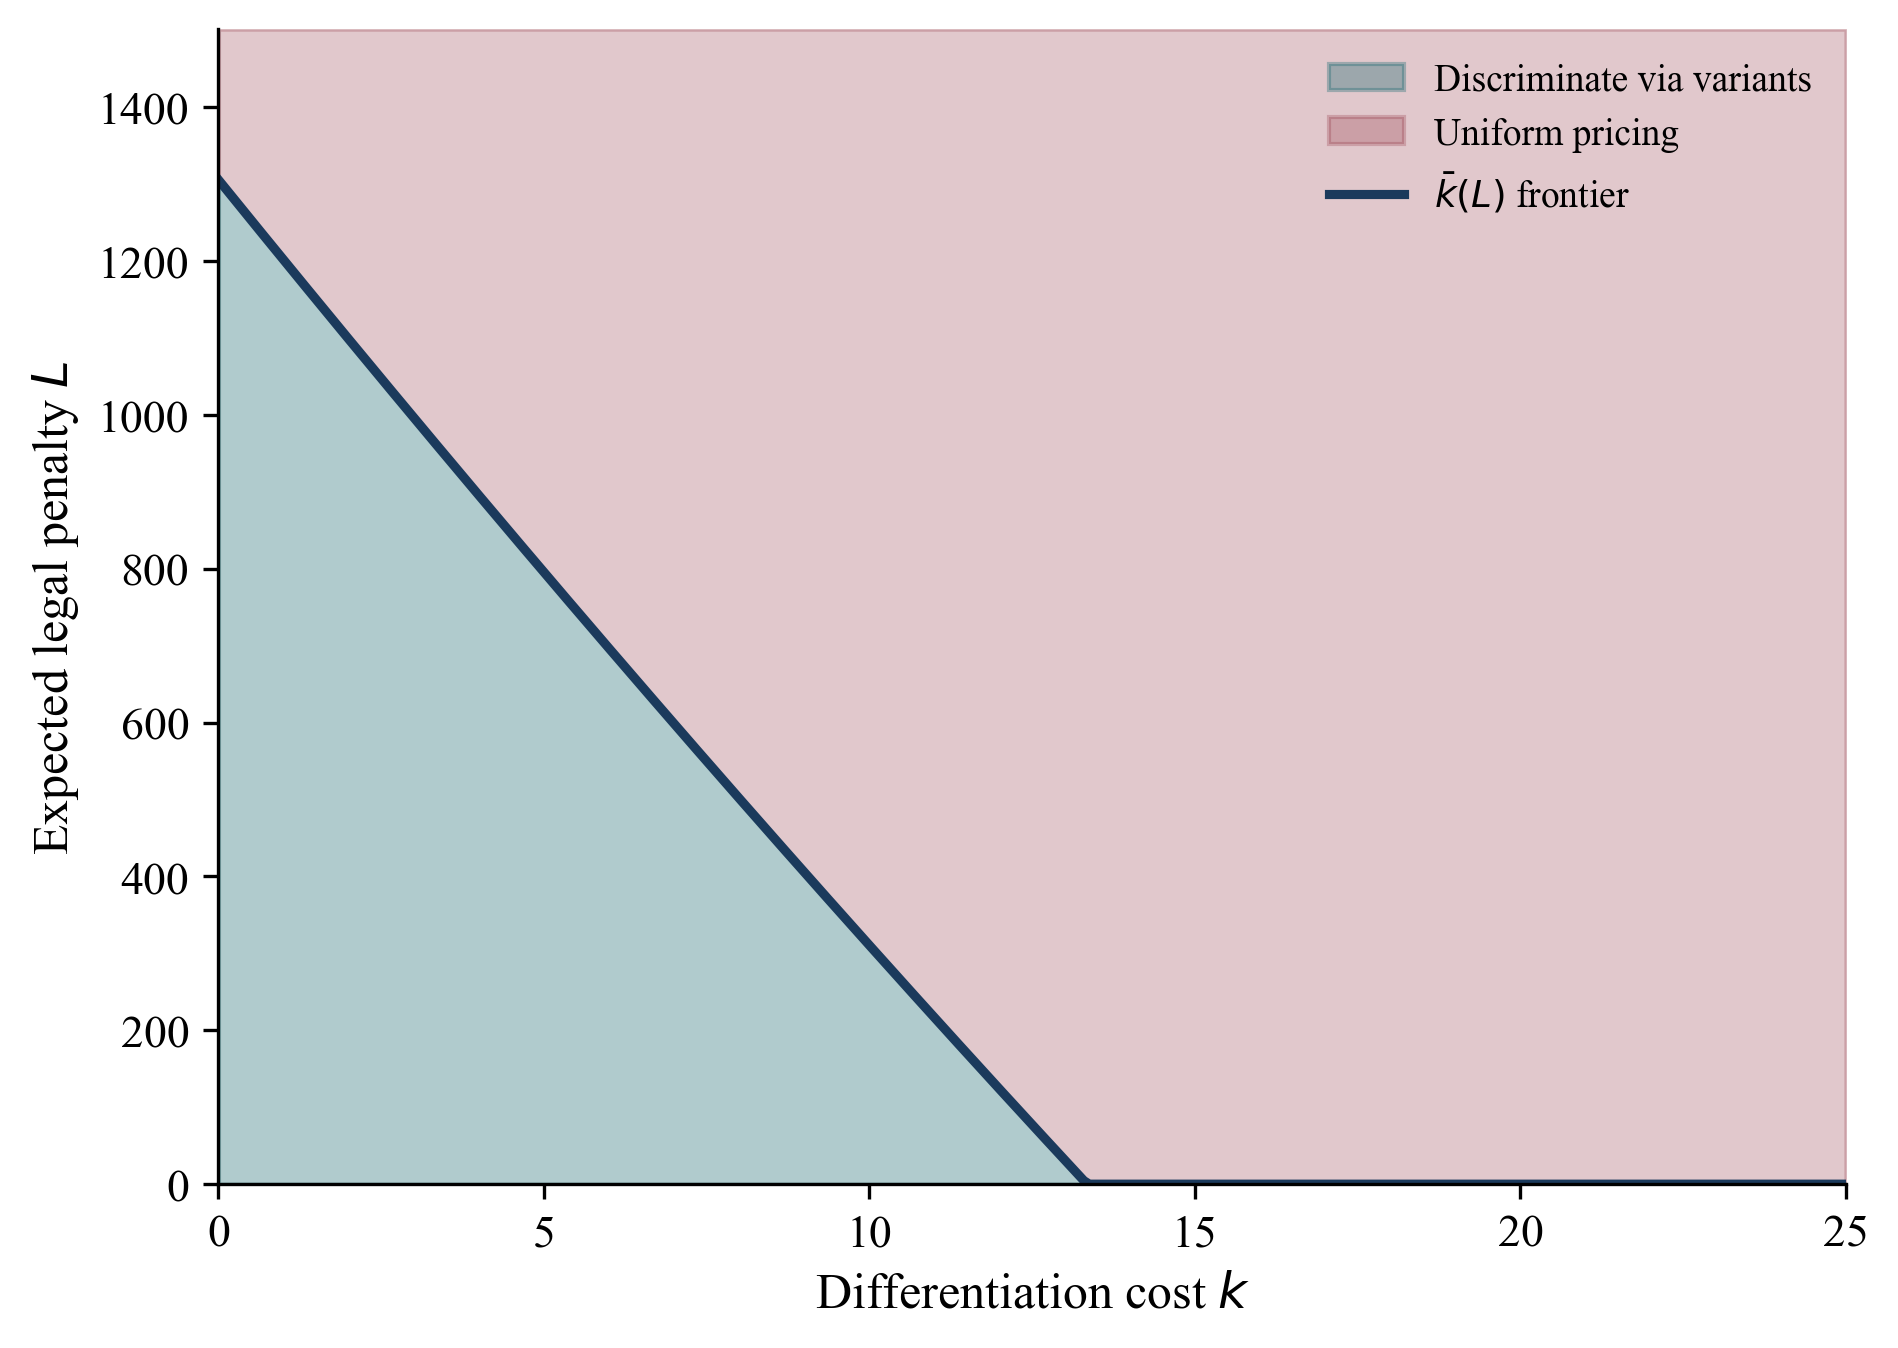
\includegraphics[width=0.75\textwidth]{fig4_kL_frontier.png}
\caption{Strategy frontier in $(k,L)$-space (\cref{prop:threshold}).
Blue region: discrimination optimal. Red region: uniform pricing dominates.}
\label{fig:kL_frontier}
\end{figure}

\begin{figure}[H]
\centering
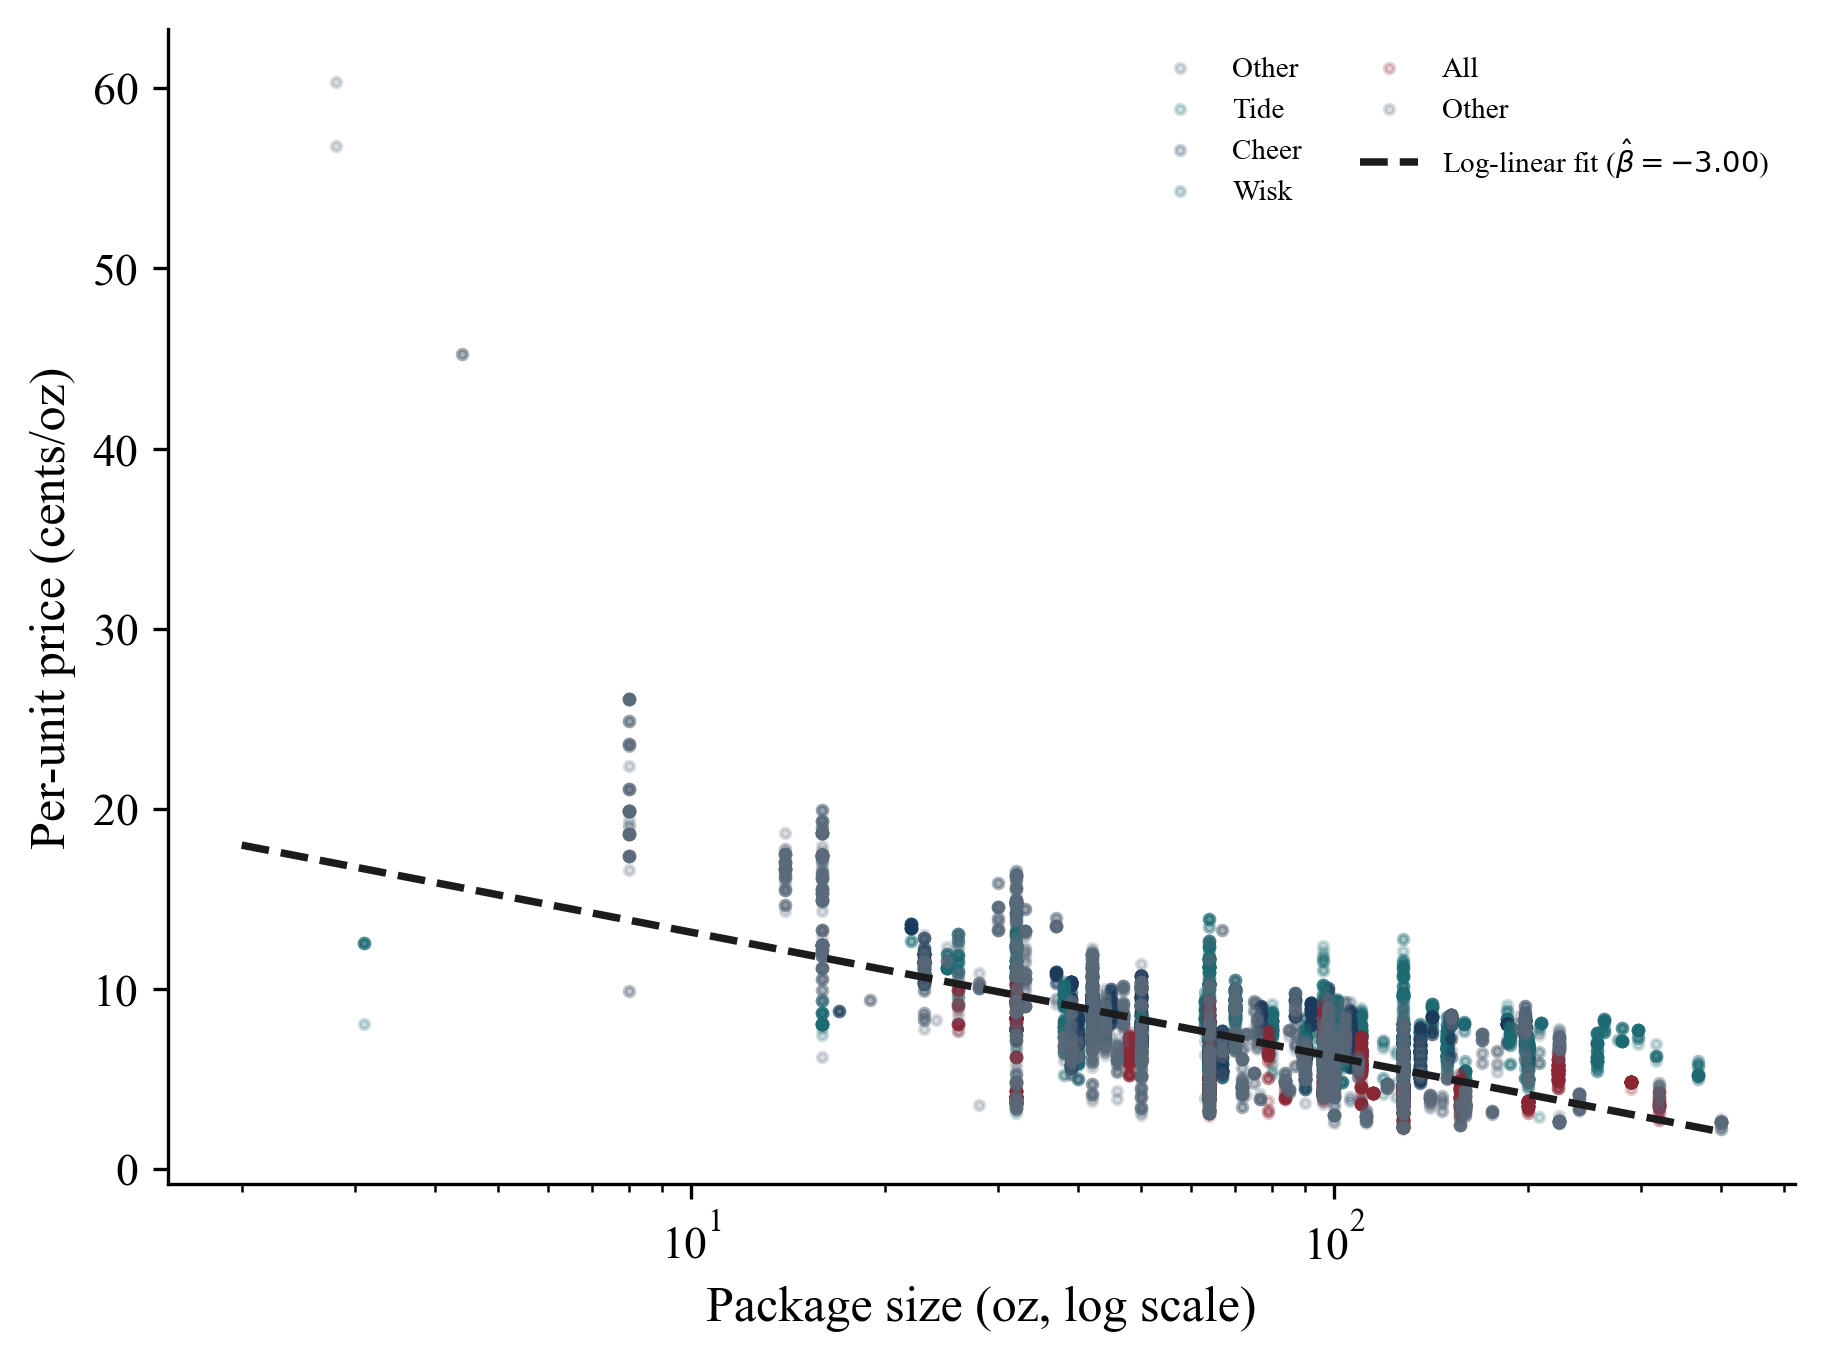
\includegraphics[width=0.75\textwidth]{fig6_size_vs_ppu.png}
\caption{Per-unit price vs.\ package size (log scale).
Points colored by brand; dashed line: log-linear fit.}
\label{fig:scatter}
\end{figure}

\begin{figure}[H]
\centering
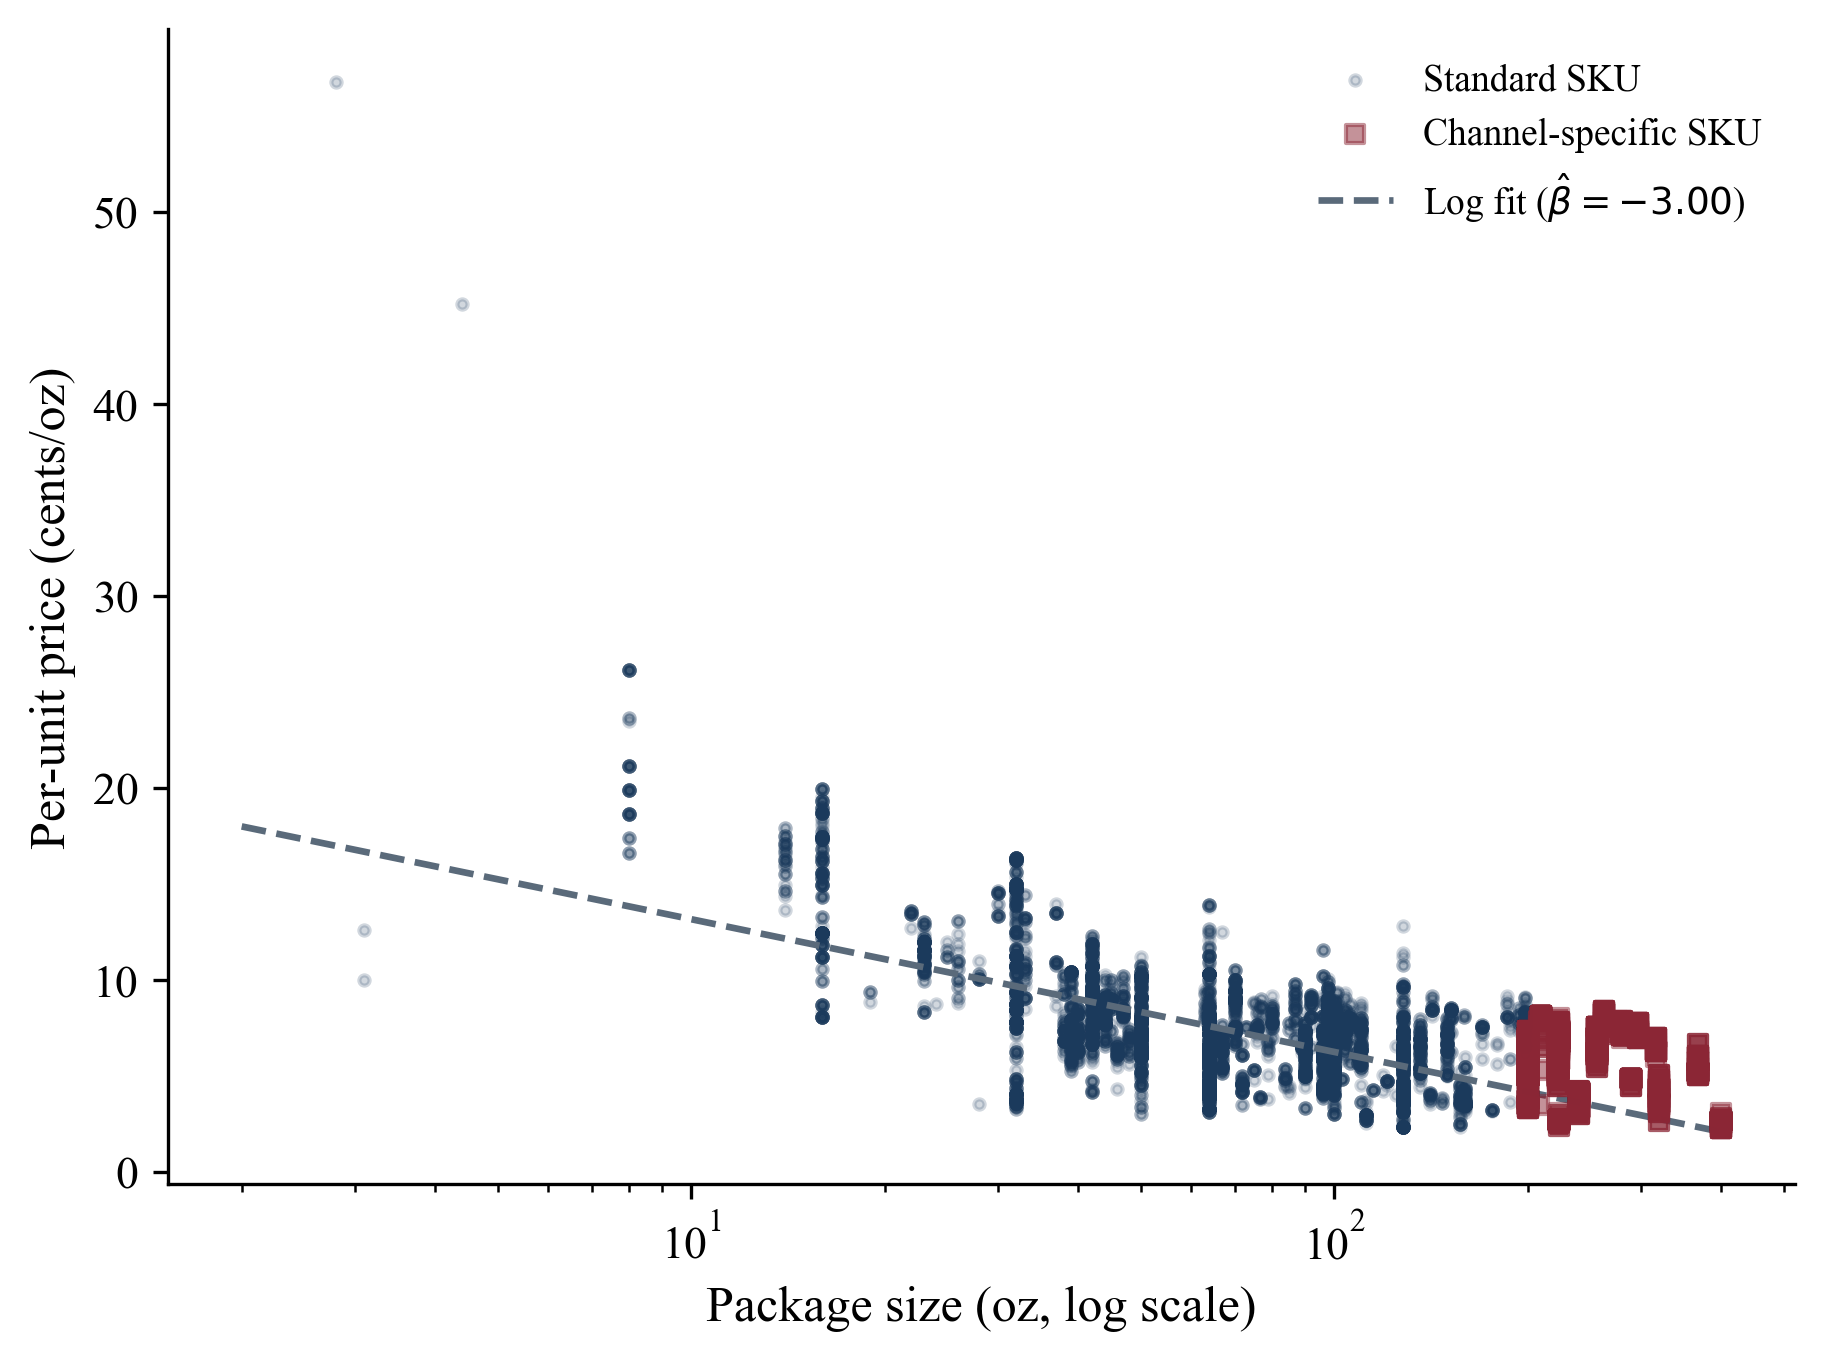
\includegraphics[width=0.75\textwidth]{fig3_scatter_channel.png}
\caption{Per-unit price vs.\ size: standard SKUs (circles) and top-5\% large-format SKUs (squares).}
\label{fig:scatter_channel}
\end{figure}

\begin{figure}[H]
\centering
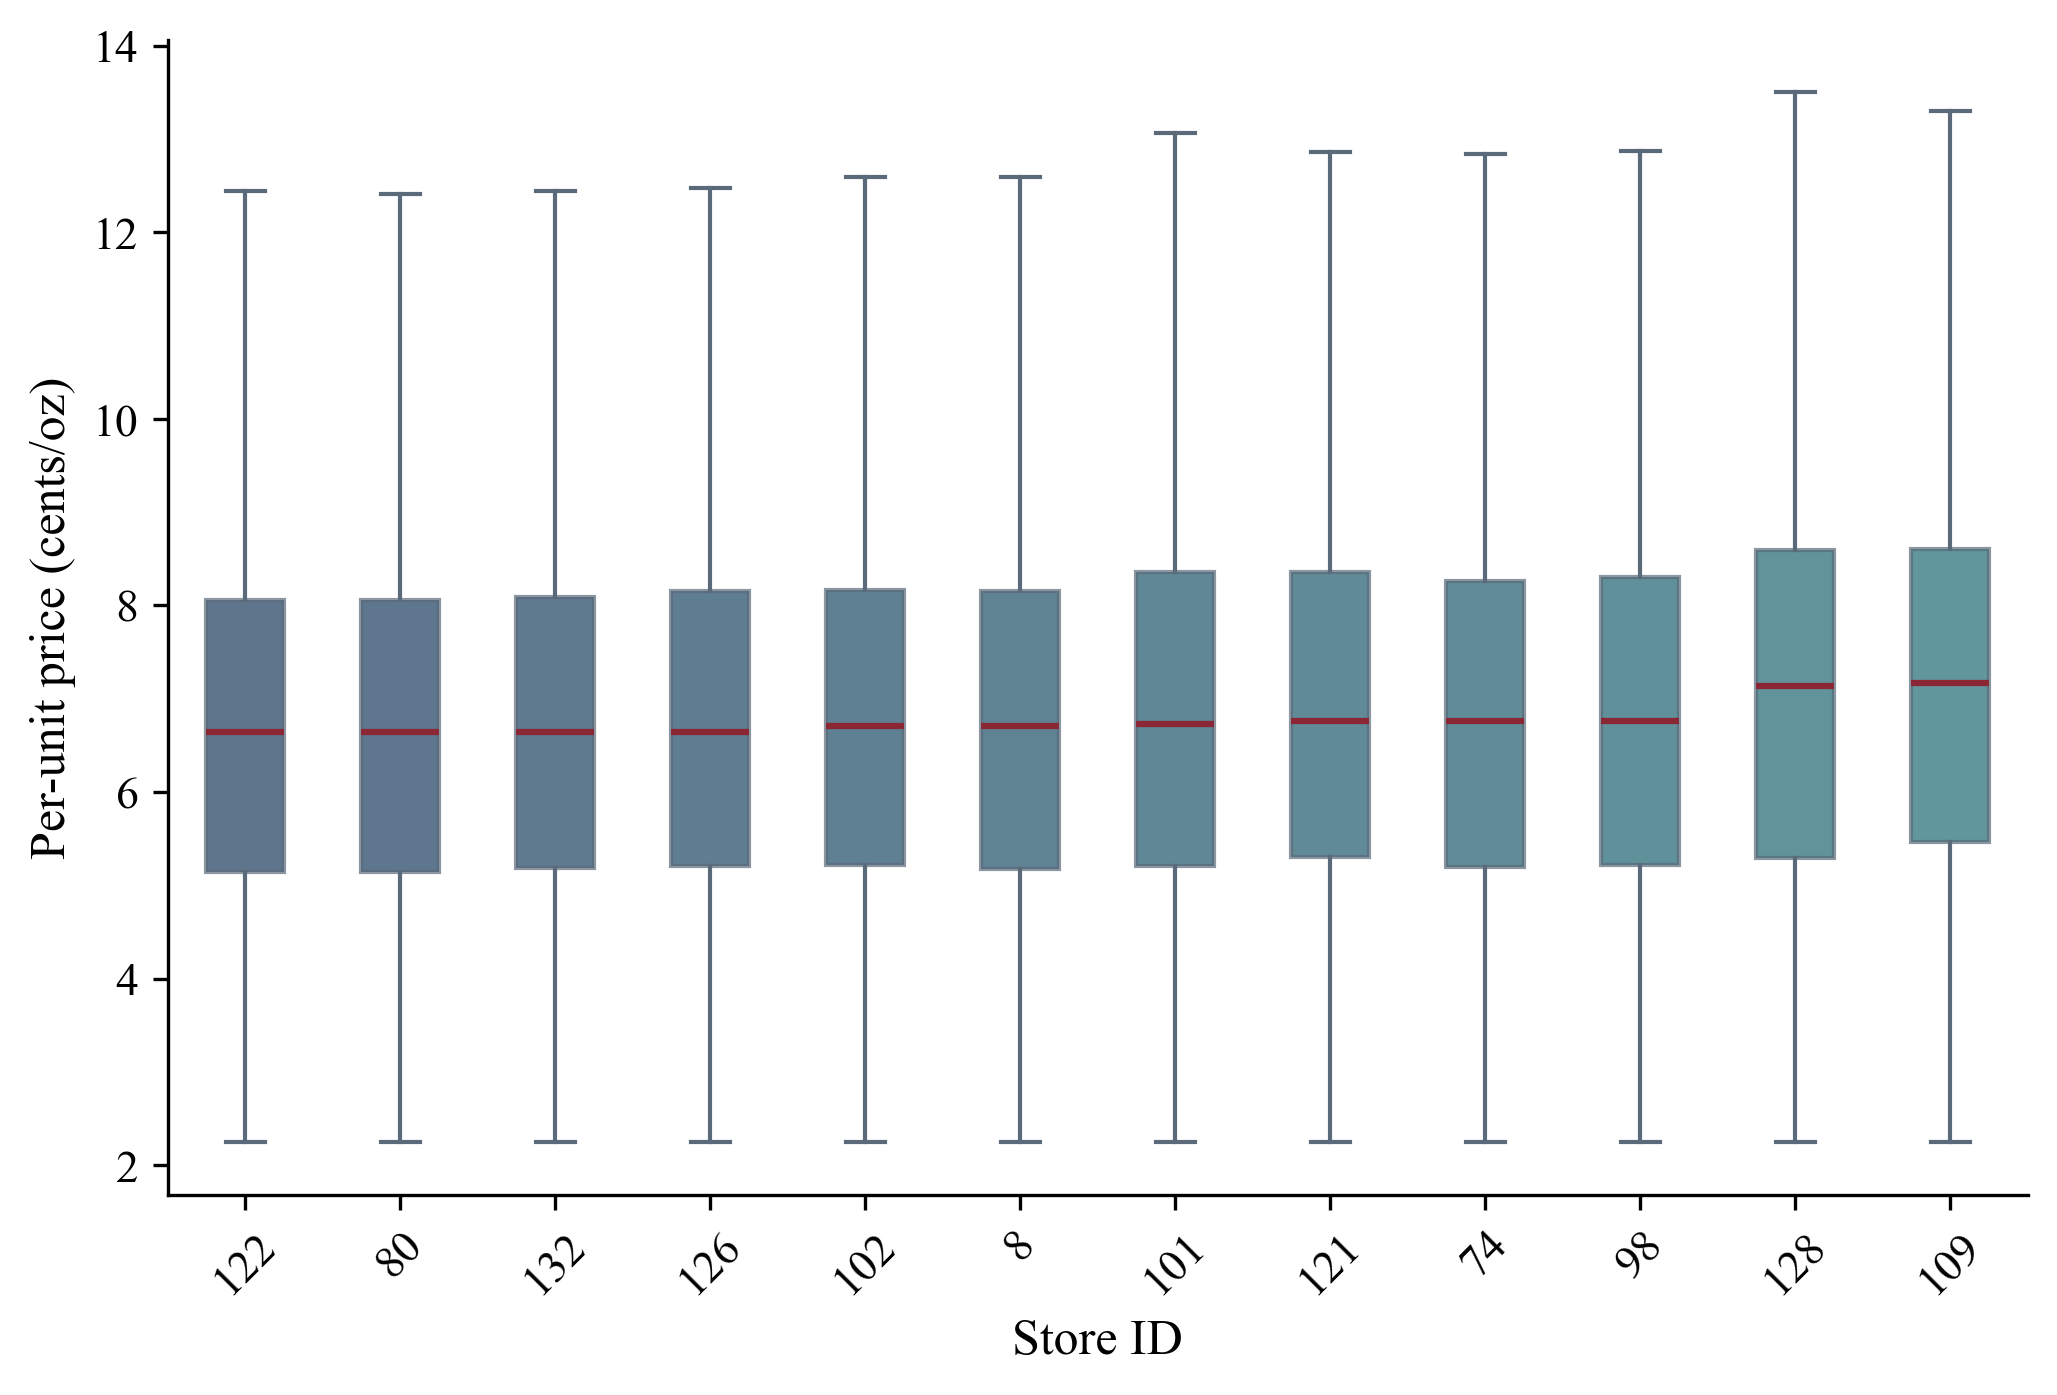
\includegraphics[width=0.75\textwidth]{fig7_ppu_by_store.png}
\caption{Per-unit price by store (12 highest-volume stores). Outliers suppressed.}
\label{fig:boxplot_store}
\end{figure}

\begin{figure}[H]
\centering
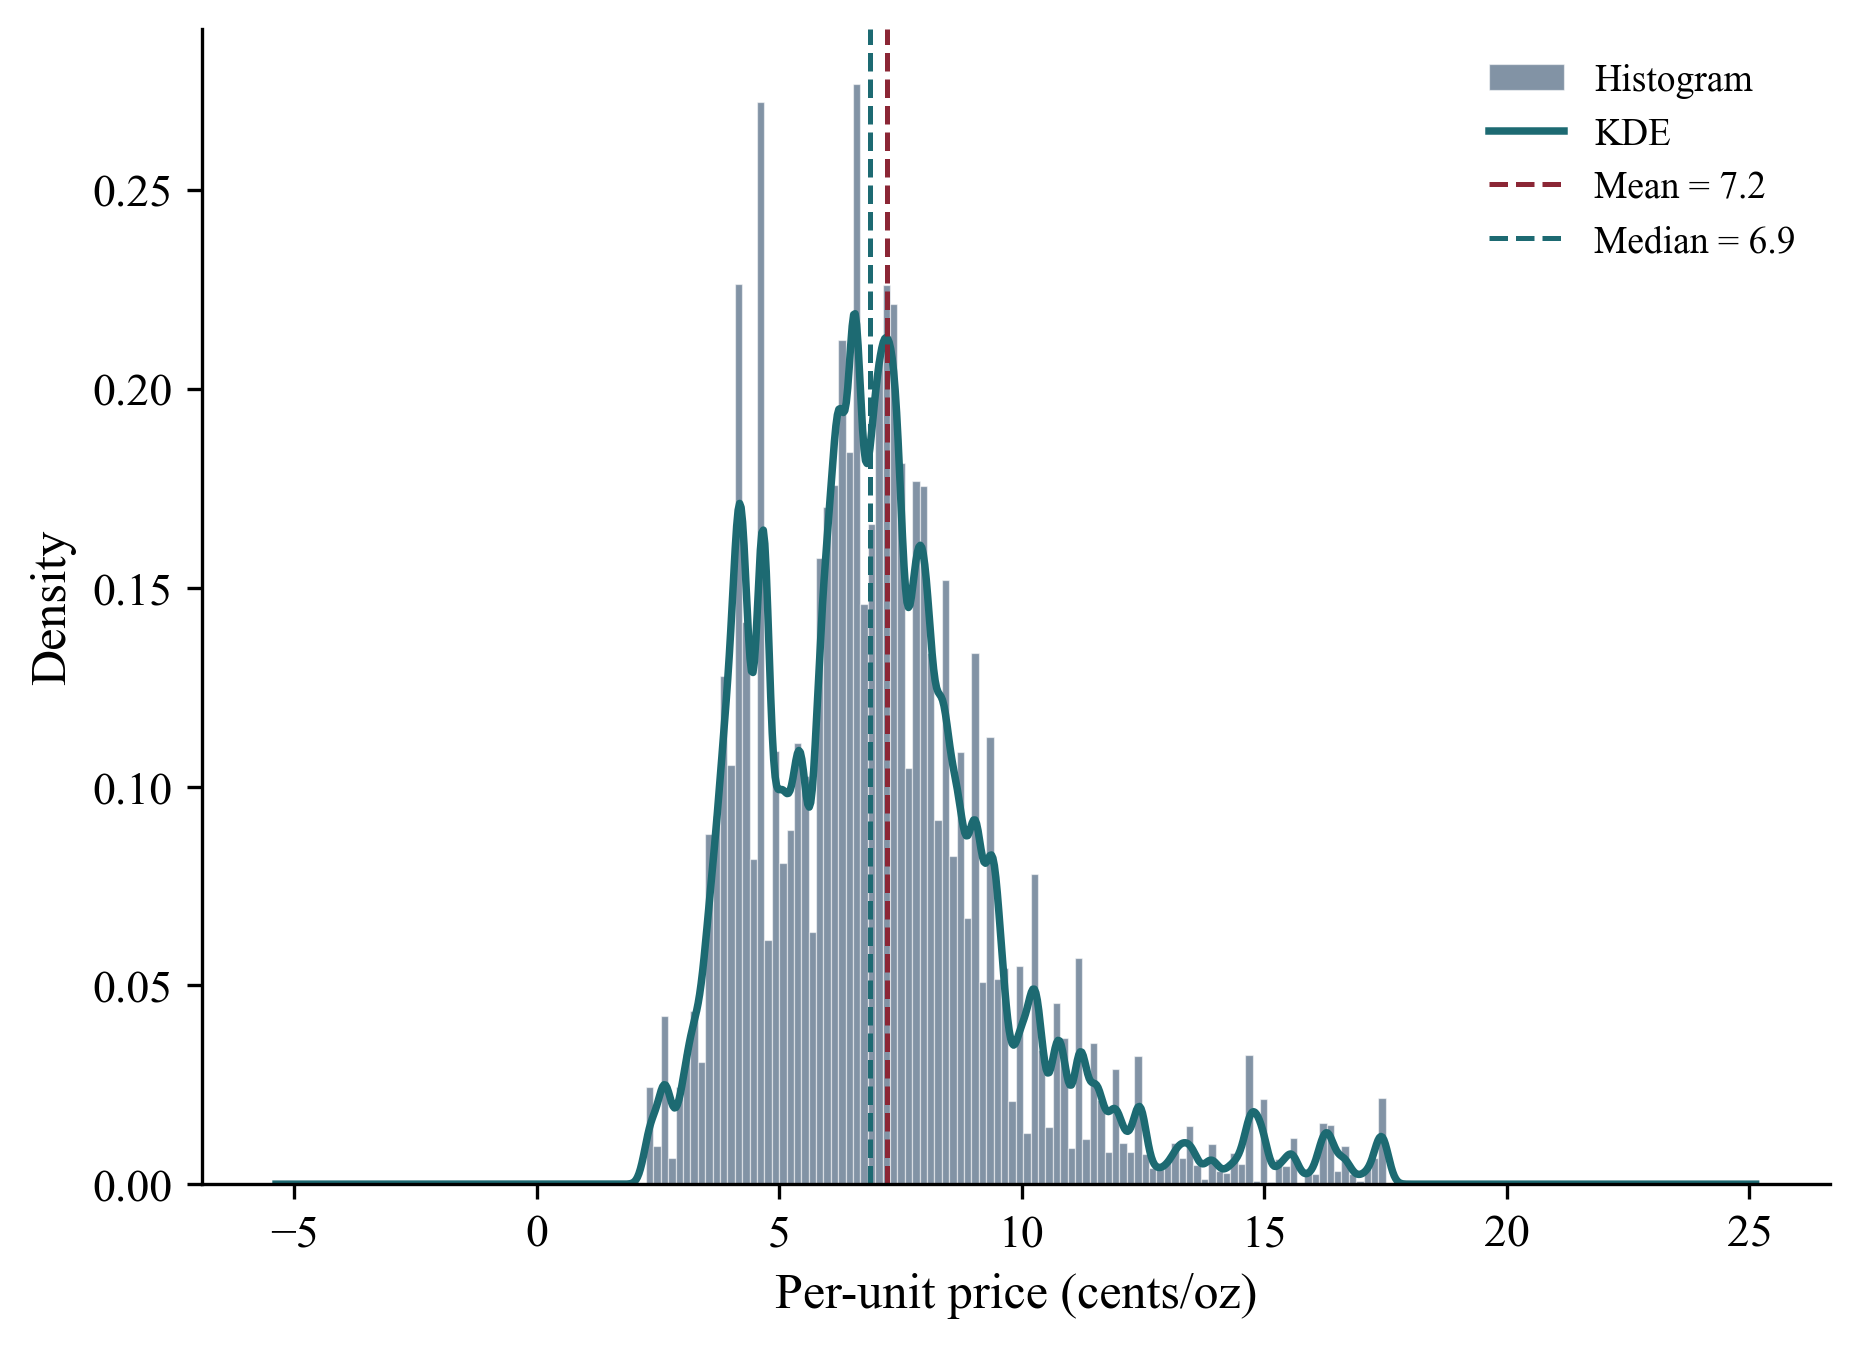
\includegraphics[width=0.75\textwidth]{fig8_ppu_distribution.png}
\caption{Distribution of per-unit prices. Vertical lines: mean and median.}
\label{fig:dist}
\end{figure}

\begin{figure}[H]
\centering
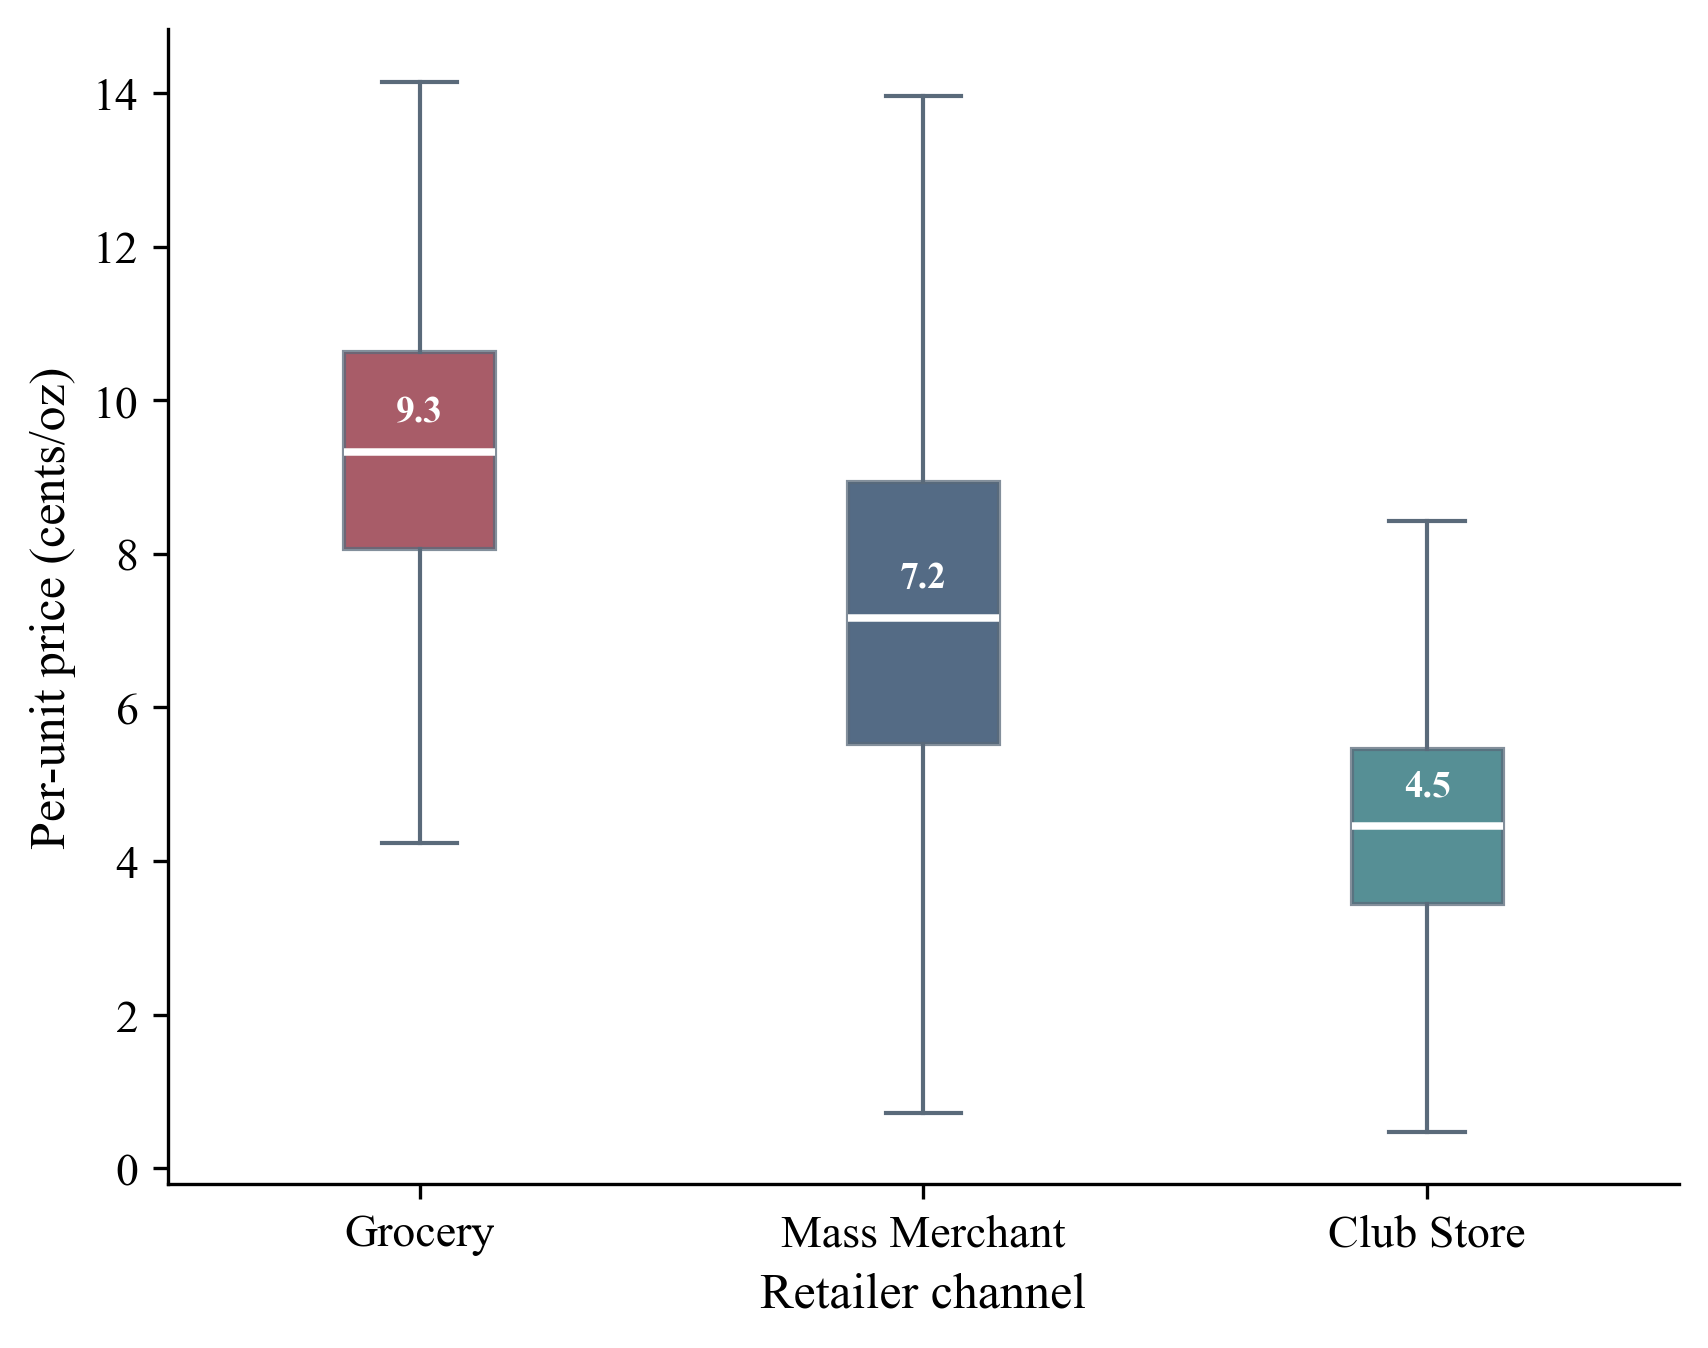
\includegraphics[width=0.65\textwidth]{fig2_retailer_boxplot.png}
\caption{Simulated cross-channel price dispersion, calibrated to Dominick's data and documented retail margins.}
\label{fig:retailer_box}
\end{figure}

\begin{figure}[H]
\centering
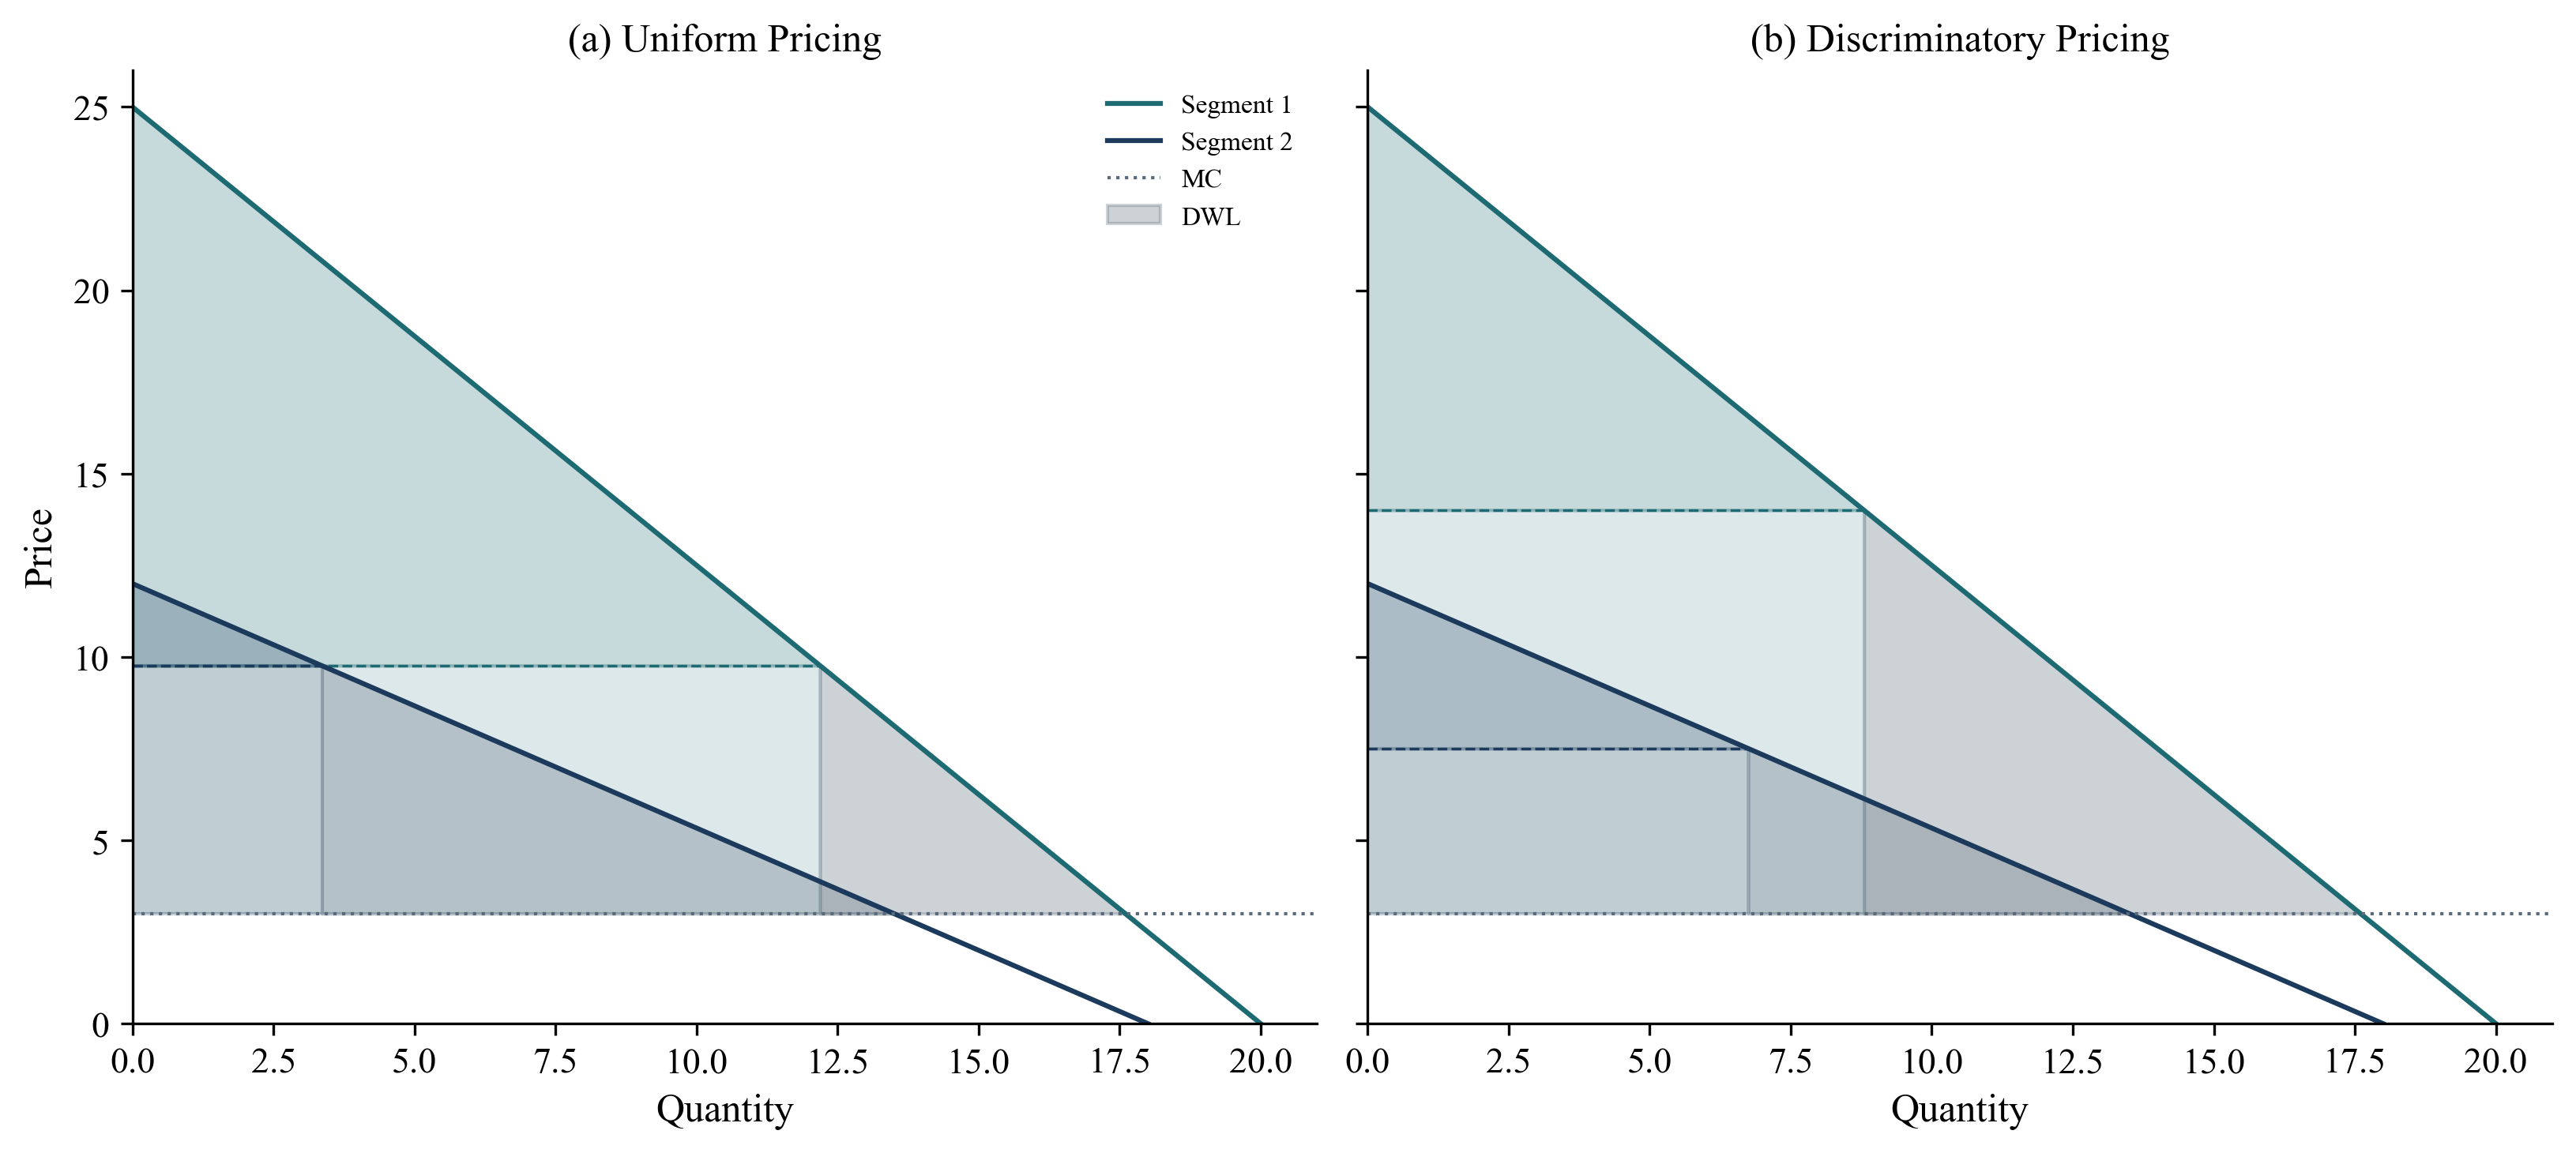
\includegraphics[width=0.9\textwidth]{fig5_welfare.png}
\caption{Welfare decomposition: (a)~uniform pricing; (b)~discriminatory pricing. Grey: deadweight loss.}
\label{fig:welfare}
\end{figure}


% ══════════════════════════════════════════════════════════════════════════
% Acknowledgements
\subsection*{Acknowledgements}
We thank the Kilts Center for Marketing (Chicago Booth) for providing the Dominick's data.
No external funding; no conflicts of interest.

\subsection*{Data availability}
The Dominick's Finer Foods dataset is publicly available at \url{https://www.chicagobooth.edu/research/kilts/research-data/dominicks}.
Replication code: \url{https://github.com/n33levo/PMandPD}.

\subsection*{AI disclosure}
Portions of this paper were drafted and revised with assistance from large-language-model tools (GitHub Copilot/Claude, OpenAI ChatGPT), used for code generation, \LaTeX{} formatting, and prose editing.
All analytical decisions were made by the authors, who take full responsibility for the manuscript.


% ══════════════════════════════════════════════════════════════════════════
\begin{thebibliography}{20}

\bibitem{Pigou1920}
A.\,C.~Pigou,
\textit{The Economics of Welfare},
Macmillan, London, 1920.

\bibitem{Varian1989}
H.\,R.~Varian,
Price discrimination,
in: R.~Schmalensee, R.~Willig (Eds.), \textit{Handbook of Industrial Organization}, vol.~1,
North-Holland, Amsterdam, 1989, pp.~597--654.

\bibitem{Schmalensee1981}
R.~Schmalensee,
Output and welfare implications of monopolistic third-degree price discrimination,
\textit{Amer.\ Econ.\ Rev.}\ \textbf{71}(1) (1981) 242--247.

\bibitem{Wilson1993}
R.\,B.~Wilson,
\textit{Nonlinear Pricing},
Oxford Univ.\ Press, 1993.

\bibitem{AdamsYellen1976}
W.\,J.~Adams, J.\,L.~Yellen,
Commodity bundling and the burden of monopoly,
\textit{Quart.\ J.\ Econ.}\ \textbf{90}(3) (1976) 475--498.

\bibitem{Yonezawa2020}
K.~Yonezawa, M.\,I.~G\'omez, T.\,J.~Richards,
The Robinson--Patman Act and vertical relationships,
\textit{Amer.\ J.\ Agric.\ Econ.}\ \textbf{102}(1) (2020) 329--352.

\bibitem{KobayashiMuris2026}
B.\,H.~Kobayashi, T.\,J.~Muris,
Stop making sense: Reviving the Robinson-Patman Act and the economics of intermediate price discrimination,
GMU/CEI Working Paper, 2026.
\url{https://papers.ssrn.com/sol3/papers.cfm?abstract_id=6299819}.

\bibitem{CBSWinners}
T.\,W.~Ross,
Winners and losers under the Robinson-Patman Act,
CBS Working Paper No.~30.
\url{https://ideas.repec.org/p/zbw/cbscwp/30.html}.

\bibitem{KhanJain2005}
R.\,J.~Khan, D.\,C.~Jain,
An empirical analysis of price discrimination mechanisms and retailer profitability,
\textit{J.\ Marketing Res.}\ \textbf{42}(4) (2005) 516--524.

\bibitem{CGM2011}
A.\,C.~Cameron, J.\,B.~Gelbach, D.\,L.~Miller,
Robust inference with multiway clustering,
\textit{J.\ Bus.\ Econ.\ Statist.}\ \textbf{29}(2) (2011) 238--249.

\bibitem{FTC_RPA}
Federal Trade Commission,
Price discrimination: Robinson-Patman violations,
\url{https://www.ftc.gov/advice-guidance/competition-guidance/guide-antitrust-laws/price-discrimination-robinson-patman-violations}.

\bibitem{Woodmans2016}
\textit{Woodman's Food Market, Inc.\ v.\ Clorox Co.}, No.~15-3001 (7th Cir.\ 2016).

\bibitem{Crowell2015}
Crowell \& Moring LLP,
Do different size packages violate the Robinson Patman Act?,
Client Alert, March 2015.

\bibitem{CrowellWoodmans2016}
Crowell \& Moring LLP,
Woodman's v.\ Clorox: Does size matter?,
Client Alert, 2016.

\bibitem{Winston2023}
Winston \& Strawn LLP,
Price discrimination claims under the resurging Robinson-Patman Act,
\textit{Competition Corner}, 2023.

\bibitem{Dominicks}
Dominick's Finer Foods Dataset,
Kilts Center for Marketing, Chicago Booth.
\url{https://www.chicagobooth.edu/research/kilts/research-data/dominicks}.

\bibitem{DominicksManual}
Dominick's Data Manual,
University of Chicago Booth School of Business.

\end{thebibliography}

\end{document}
